\section{funzioni}

Sia $f$ una relazione tra due insiemi $A$ e $B$. 
Useremo la notazione delle frecce quindi scriveremo $a\stackrel f\mapsto b$ 
se $(a,b)\in f$. 
Diremo che $f$ è una funzione da $A$ in $B$ e scriveremo 
$f\colon A\to B$ se per ogni $a\in A$ esiste un unico $b\in B$ 
tale che $a \stackrel f \mapsto b$.
Potremmo dire che $f$ è definita su $A$ 
(perché per ogni punto $a$ in $A$ c'è una freccia uscente da $a$)
ed è univoca (perché tale freccia è unica).

Dato $a\in A$ esiste dunque un unico $b\in B$ tale che
$a\stackrel f \mapsto b$: chiameremo $fa$
o $f(a)$ 
\mymargin{$f(x)$}%
tale oggetto $b$
e diremo che la funzione $f$ manda $a$ in $b$. 
Si avrà dunque
\[
 b=f(a) \iff a\stackrel f \mapsto b.
\]
Gli elementi del dominio spesso vengono chiamati \emph{punti}
mentre gli elementi del codominio vengono 
chiamati \emph{valori}. 
La funzione $f$ avrà quindi valore $f(a)$ nel punto $a$.
L'insieme di tutte le funzioni $f\colon A\to B$ viene usualmente denotato $B^A$
oppure $A\to B$.
\mymargin{$B^A$}%
\index{$A^B$}%
\index{$A\to B$}%
\index{potenza!insiemi}%

\begin{figure}
  \mbox{}
  \hfill
  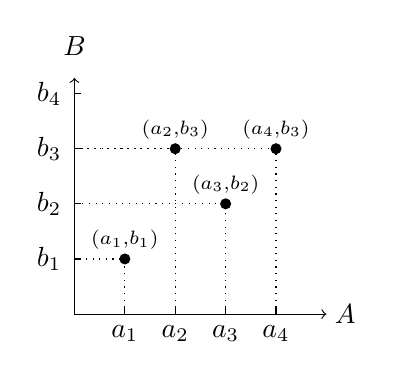
\begin{tikzpicture}[x=0.8cm]
  	\draw[->] (0,0) -- (4,0);
  	\draw[->] (0,0) -- (0,3.0);
  	\node at (4.3,0) {$A$};
  	\node at (0,3.4) {$B$};

      \draw (0.8,0) -- +(0,0.1) node [label=below:$a_1$]{};
      \draw (1.6,0) -- +(0,0.1) node [label=below:$a_2$]{};
      \draw (2.4,0) -- +(0,0.1) node [label=below:$a_3$]{};
      \draw (3.2,0) -- +(0,0.1) node [label=below:$a_4$]{};

      \draw (0,0.7) -- +(0.1,0) node [label=left:$b_1$]{};
      \draw (0,1.4) -- +(0.1,0) node [label=left:$b_2$]{};
      \draw (0,2.1) -- +(0.1,0) node [label=left:$b_3$]{};
      \draw (0,2.8) -- +(0.1,0) node [label=left:$b_4$]{};

  	\draw[dotted] (0.8,0) -- (0.8,0.7) -- (0,0.7);
  	\draw[dotted] (1.6,0) -- (1.6,2.1) -- (0,2.1);
  	\draw[dotted] (2.4,0) -- (2.4,1.4) -- (0,1.4);
  	\draw[dotted] (3.2,0) -- (3.2,2.1) -- (0,2.1);

  	\fill (0.8,0.7) circle (2pt) node[above] {$\scriptstyle (a_1,b_1)$};
  	\fill (1.6,2.1) circle (2pt) node[above] {$\scriptstyle (a_2,b_3)$};
  	\fill (2.4,1.4) circle (2pt) node[above] {$\scriptstyle (a_3,b_2)$};
  	\fill (3.2,2.1) circle (2pt) node[above] {$\scriptstyle (a_4,b_3)$};
  \end{tikzpicture}
\hfill
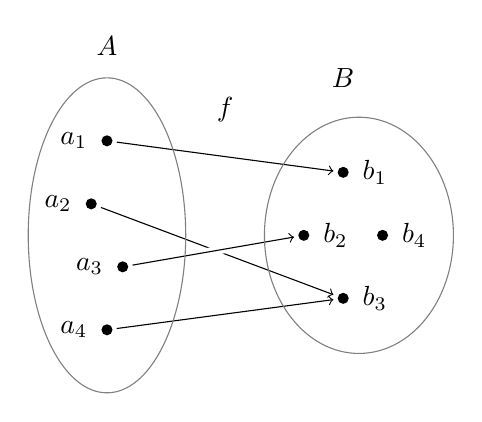
\begin{tikzpicture}[x=1cm,y=0.8cm]
\fill (1,4) circle (2pt) node (a1) [label=left:$a_1$]{};
\fill (0.8,3) circle (2pt) node (a2) [label=left:$a_2$]{};
\fill (1.2,2) circle (2pt) node (a3) [label=left:$a_3$]{};
\fill (1,1) circle (2pt) node (a4) [label=left:$a_4$]{};
\fill (4,3.5) circle (2pt) node (b1) [label=right:$b_1$] {};
\fill (3.5,2.5) circle (2pt) node (b2) [label=right:$b_2$] {};
\fill (4,1.5) circle (2pt) node (b3) [label=right:$b_3$] {};
\fill (4.5,2.5) circle (2pt) node (b4) [label=right:$b_4$] {};
\draw[->] (a1) edge (b1);
\draw[->] (a2) edge (b3);
\draw[line width=3pt,white] (a3) edge (b2);
\draw[->] (a3) edge (b2);
\draw[->] (a4) edge (b3);
\draw[draw=gray](1,2.5) ellipse (1cm and 2cm);
\draw[draw=gray](4.2,2.5) ellipse (1.2cm and 1.5cm);
\node at (1,5.5) {$A$};
\node at (4,5) {$B$};
\node at (2.5,4.5) {$f$};
\end{tikzpicture}
\hfill
\mbox{}
\caption[]{La funzione $f\colon A\to B$,
$f=\{a_1\mapsto b_1,$ $a_2 \mapsto b_3,$ $a_3 \mapsto b_2,$ $a_4 \mapsto b_3\}$
definita sull'insieme $A=\ENCLOSE{a_1, a_2, a_3, a_4}$
a valori nell'insieme $B=\ENCLOSE{b_1, b_2, b_3, b_4}$
rappresentata tramite grafico e
tramite diagrammi di Venn.}
\label{fig:funzione}
\end{figure}

L'insieme di partenza $A$ viene chiamato \emph{dominio}%
\mymargin{dominio}%
\index{dominio} 
della funzione $f\colon A\to B$,
mentre l'insieme di arrivo $B$ viene chiamato \emph{codominio}%
\mymargin{codominio}%
\index{codominio}.
La funzione $f$ rappresenta quindi un modo di assegnare in maniera univoca
ad ogni elemento del dominio un elemento del codominio.
Da un punto di vista informatico potremmo dire che $A$ è l'insieme
dei possibili \emph{input} e $B$ è l'insieme dei possibili \emph{output}
della funzione $f$.

Per come l'abbiamo definita, una funzione è dunque un insieme.
In generale le funzioni potrebbero essere definite in altri modi oppure 
potrebbero essere un concetto primitivo: dunque nei capitoli seguenti useremo le funzioni 
senza assumere che esse siano a loro volta degli insiemi.
Ad esempio invece di scrivere $(a,b)\in f$ scriveremo sempre $f(a)=b$ 
oppure $a\stackrel f \mapsto b$.
Sarà comunque molto importante
considerare l'insieme che rappresenta $f$ ma questo verrà chiamato
\emph{grafico}%
\mymargin{grafico}%
\index{grafico} di $f$, $G_f$ e potrà essere definito in questo modo:
\[
  G_f = \ENCLOSE{(x,y)\in A \times B\colon f(x)=y}.
\]
Nella nostra costruzione risulta effettivamente $G_f = f$ ma, come abbiamo detto,
in generale è opportuno distinguere la funzione dal suo grafico.
Uno degli argomenti principali di questo corso è lo studio 
del grafico delle funzioni reali, cioè le funzioni 
con dominio e codominio nell'insieme dei numeri reali.

\subsection{invertibilità}

Capita molto spesso che un fenomeno possa essere modellizzato matematicamente
tramite una funzione: si sa che ad un certo \emph{input} $a$ corrisponde
un \emph{output} $b=f(a)$. Molto spesso il problema da risolvere è
quello di determinare l'\emph{input} giusto $a$ per ottenere l'\emph{output}
voluto $b$. Questo problema corrisponde ad \emph{invertire} la funzione $f$:
dato $b\in B$ determinare $x\in A$ tale che $f(x) = b$.

Una funzione $f\colon A \to B$ si dice essere \emph{surgettiva}%
\mymargin{surgettiva}%
\index{surgettiva} (o \emph{suriettiva})
se per ogni $b\in B$ esiste almeno un $x\in A$ per cui $f(x)=b$. Questo
significa che il problema dell'inversione ha almeno una soluzione, qualunque
sia $b\in B$.
Una funzione $f\colon A \to B$ si dice essere \emph{iniettiva}%
\mymargin{iniettiva}%
\index{iniettiva}
se non esistono due punti distinti $a,a' \in A$, $a\neq a'$ tali
che $f(a) = f(a')$. Questo significa che il problema dell'inversione
$f(x)=b$ ha al più una soluzione (la soluzione, se esiste, è unica).
Una funzione $f\colon A \to B$ si dice essere \emph{bigettiva}%
\mymargin{bigettiva}%
\index{bigettiva}
(o \emph{biettiva})
\index{biettiva}%
\index{bigettiva}%
\index{funzione!bigettiva}%
\index{invertibile}%
\index{funzione!invertibile}%
\index{biettiva}%
o
\emph{invertibile}%
\mymargin{invertibile}%
\index{invertibile}%
\mynote{\textbf{Attenzione:} in alcuni testi (tra cui~\cite{Giusti}) si considerano
invertibili le funzioni iniettive, anche se non surgettive.}
se è sia iniettiva che surgettiva. Questo significa
che il problema dell'inversione $f(x)=b$ ha una unica soluzione $x\in A$
qualunque sia $b\in B$. In particolare, se $f$ è invertibile, per ogni $b\in B$ esiste
un unico $a\in A$ per cui $f(a)=b$.
Se $f$ è una funzione invertibile allora la relazione inversa $g$
cioè la relazione tale che $b\stackrel g \mapsto a$ quando $a \stackrel f \mapsto b$
risulta essere una funzione $g\colon B\to A$. 
Infatti $g$ è definita su tutto $B$ in quanto $f$ è surgettiva 
e $g$ è univoca in quanto $f$ è iniettiva.
Le proprietà caratteristiche della \emph{funzione inversa}%
\mymargin{funzione inversa}%
\index{funzione!inversa} $g$ sono:
\begin{equation}\label{eq:572098}
  \forall a\in A\colon g(f(a)) = a, \qquad
  \forall b\in B\colon f(g(b)) = b.
\end{equation}
La funzione $g$ inversa di $f$ viene usualmente denotata con il simbolo $f^{-1}$.

Se $f\colon A\to B$ è bigettiva diremo che $A$ 
e $B$ sono in \emph{corrispondenza biunivoca}%
\mymargin{corrispondenza biunivoca}%
\index{corrispondenza!biunivoca} tramite $f$.
In effetti $f$ è una corrispondenza \emph{univoca} da $A$ in $B$
(manda in modo univoco ogni punto di $A$ in un punto di $B$)
e $f^{-1}$ è una corrispondenza univoca da $B$ in $A$.

Introduciamo ora delle notazioni che sarà comodo utilizzare nel seguito.
Se $f\colon A \to B$ è una funzione e se $C\subset A$ definiamo
\[
  f(C) 
  = \ENCLOSE{f(a)\colon a \in C} 
  = \ENCLOSE{b\in B\colon \exists a\in C\colon b=f(a)}.
\]
L'insieme $f(C)\subset B$ si chiama \emph{immagine}%
\mymargin{insieme immagine}%
\index{immagine}
\index{immagine!insieme}%
di $C$ (tramite $f$) ed è formato
da tutti i punti che si ottengono applicando $f$ agli elementi di $C$.
L'immagine $f(A)$ dell'intero dominio $A$ si chiama immagine di $f$
e si denota a volte con il simbolo $\Im f$.
Si noti che $f$ è surgettiva se e solo se $f(A)=B$ (cioè se l'immagine coincide
col codominio).
Ad esempio la funzione definita in Figura~\ref{fig:funzione}
ha immagine $f(A) = \ENCLOSE{f(a_1),f(a_2),f(a_3),f(a_4)} 
 = \ENCLOSE{b_1, b_2, b_3}$.

Anche se $f\colon A \to B$ non fosse iniettiva,
per ogni $C\subset B$ possiamo definire
\[
  f^{-1}(C) = \ENCLOSE{a\in A\colon f(a) \in C}.
\]
L'insieme $f^{-1}(C)\subset A$ si chiama \emph{preimmagine}
o \emph{controimmagine}
\mymargin{preimmagine}%
\index{preimmagine}%
\index{preimmagine!insieme}%
\index{controimmagine!insieme}%
\index{insieme!controimmagine}%
di $C$ (tramite $f$)
ed è formato da tutti i punti di $A$ che applicando $f$ vanno in $C$.
Si noti che se $b\in B$ l'insieme $f^{-1}(\ENCLOSE{b})$ non è altro che
l'insieme delle soluzioni dell'equazione $f(x)=b$. Come abbiamo
già visto tale insieme contiene almeno un elemento se $f$ è suriettiva,
contiene al più un elemento se $f$ è iniettiva e contiene esattamente
un elemento $f^{-1}(\ENCLOSE{b}) = \ENCLOSE{f^{-1}(b)}$ se $f$ è bigettiva.
Ad esempio se $f$ è la funzione definita in figura~\ref{fig:funzione}
si ha $f^{-1}(\ENCLOSE{b_3,b_4}) = f^{-1}(\ENCLOSE{b_3}) = \ENCLOSE{a_2,a_4}$,
$f^{-1}(\ENCLOSE{b_4}) = \emptyset$.


La notazione $f(C)$ appena introdotta è formalmente ambigua in quanto
potrebbe non essere chiaro se $C$ è un elemento oppure un sottoinsieme
del dominio di $f$.
In pratica il contesto dovrebbe rendere chiaro cosa si intende.

Più in generale ci capiterà di estendere questo abuso di notazione non solo
alle funzioni, ma anche alle relazioni e alle operazioni.
Ad esempio se $A$ e $B$ sono insiemi di numeri ci capiterà di scrivere $A\le B$
per intendere che ogni elemento di $A$ è minore o uguale ad ogni elemento di $B$
oppure $A+B$ per intendere l'insieme di tutti i numeri che si ottengono sommando
ogni numero elemento di $A$ ad ogni numero elemento di $B$.

\begin{exercise}
  Sia $f\colon A \to B$ una funzione qualunque. 
  Si verifichi che se $C\subset A$ e $D\subset B$ si ha 
  \[
    f^{-1}(f(C))\supset C,
    \qquad 
    f(f^{-1}(D)) \subset D. 
  \]
  
  Che ipotesi possiamo fare su $f$ per avere l'uguaglianza
  $f(f^{-1}(C)) = C$?
  E per avere $f^{-1}(f(D)) = D$?
\end{exercise}

Si osservi che se $f\colon A \to B$ è una funzione e 
se $C\supset f(A)$ allora risulta anche $f\colon A \to C$ in quanto 
i valori di $f$ sono elementi di $C$. 
Dunque il \emph{codominio} di una 
funzione può essere esteso o ristretto con l'accortezza di mantenere 
tutti i valori dell'immagine. 
In particolare $f\colon A \to f(A)$ è certamente surgettiva.

Ad esempio vedremo che la funzione $\sin$ 
sarà definita con dominio l'insieme $\RR$ dei numeri reali 
ma può avere come codominio sia $\RR$ stesso
che solamente l'intervallo $[-1,1]$ dei numeri compresi 
tra $-1$ e $1$. 
Non ha quindi senso chiedersi se $\sin$ è suriettiva finché 
non dichiaro qual è il codominio considerato:
$\sin\colon \RR\to[-1,1]$ è suriettiva mentre 
$\sin\colon \RR\to\RR$ non lo è. 
Altri testi considerano il codominio parte della definizione 
della funzione e quindi considerano diverse due funzioni 
che hanno lo stesso grafico ma codominio diverso. 
E' una sottigliezza di poca rilevanza.

Per rendere iniettiva una funzione dobbiamo invece restringere il dominio.

\begin{definition}[restrizione]
  \label{def:restrizione}%
  Se $f\colon A\to B$ è una funzione e $C\subset A$, possiamo 
  \emph{restringere} il dominio di $f$ all'insieme $C$.
  \mynote{La notazione $f\llcorner C$ non è del tutto standard,
  probabilmente è più comune la notazione $f_{|C}$.}%
  Si ottiene una nuova funzione $f\llcorner C$ che coincide con $f$
  ma che è definita solo su $C$: $f\llcorner C\colon C\to B$:
  \[
  f\llcorner C(x) = f(x)\qquad 
  \forall x \in C.
  \]
\end{definition}


\subsection{funzione composta}
\index{composizione!di funzioni}%

Se $f\colon A\to B$ e $g\colon B\to C$ allora un punto $a\in A$ 
viene mandato tramite $f$ in un punto $b\in B$ e 
a sua volta il punto $b$ viene mandato da $g$ in un punto 
$c \in C$. 
La funzione che manda $a$ in $c$ viene chiamata 
\emph{funzione composta}%
\mymargin{funzione composta}%
\index{funzione!composta} si denota con $g\circ f$ 
e si può definire così:
\[
g\circ f \colon A \to C, \qquad 
(g\circ f)(x) = g(f(x)).  
\]

Se abbiamo tre funzioni 
$f\colon A\to B$, $g\colon B\to C$ e $h\colon C\to D$ 
allora è facile verificare che:
\[
   h \circ (g\circ f) = (h\circ g) \circ f
\]
in quanto per ogni $x\in A$ si ha
\[
(h \circ (g\circ f)) (x) =
h(g(f(x))) = (h\circ g)(f(x)) = ((h\circ g) \circ f) (x).  
\]
Significa che l'operatore di composizione $\circ$
soddisfa la proprietà associativa.

Se $f\colon A\to B$ è bigettiva allora 
per ogni $x\in A$ e per ogni $y\in B$ si ha,
grazie a~\eqref{eq:572098},
\[
  f^{-1} (f(x)) = x,
  \qquad f(f^{-1}(y)) = y.
\]
Significa che 
\[
  f^{-1}\circ f = \id_A, 
  \qquad
  f\circ f^{-1} = \id_B
\] 
dove $\id_X\colon X\to X$
è la funzione 
\emph{identità}%
\mymargin{identità}%
\index{identità} 
\index{funzione!identità}%
cioè la funzione 
che lascia fisso ogni punto di $X$:
\mymargin{$\id_X$}%
\index{$\id$}%
\[
\id_X(x) = x \qquad \text{per ogni $x\in X$}.
\]

\begin{theorem}
Se $f\colon A\to B$ e $g\colon B\to C$ sono entrambe invertibili
anche $g\circ f\colon A\to C$ è invertibile e si ha 
\begin{equation}\label{eq:inversa_composta}
  (g\circ f)^{-1} = f^{-1}\circ g^{-1}.
\end{equation}
\end{theorem}
\begin{proof}    
Per ogni $c\in C$ esiste un unico $b\in B$ tale che $g(b)=c$ 
ed un unico $a\in A$ tale che $f(a)=b$. 
Tale $a$ è l'unico punto per cui $g(f(a))=c$ e questo dimostra che 
$g\circ f$ è bigettiva. Inoltre $a=f^{-1}(b)$ e $b=g^{-1}(c)$ 
dunque $(g\circ f)^{-1}(c) = a = f^{-1}(g^{-1}(c))$ da cui si ottiene 
\eqref{eq:inversa_composta}.
\end{proof}

\begin{exercise}
  Si verifichi che la composizione di funzioni iniettive è iniettiva e la composizione 
  di funzione suriettive è suriettiva.
\end{exercise}

